% !TeX root = ../../Book3.tex
% 纲要标题：### 16.2 短时热核的局部构造
% 纲要位置：几何学计划纲要.md，第 2758 行。
% 正文状态：初稿；尚未正式审核。

% 纲要内容开始
% 
% * 测地距离和 Gaussian 主项
% * 运输方程与系数递推
% * 截断参数核的误差
% * Volterra 修正及余项控制
% * 局部构造与谱核的一致性
% 
% 纲要内容结束

\section{短时热核的局部构造}
\label{g3:sec:1602}

热核在时间很小时主要集中于距离约为 \(\sqrt t\) 的范围。这个尺度上，切空间中的 Gaussian 核给出主项，度量及其导数则进入逐阶修正。本节从这些局部数据构造一个近似核，再用收敛的时间卷积级数消去误差。最后借上一节的唯一性识别所得核，并证明可逐阶求导的统一余项。

\subsection{测地距离和 Gaussian 主项}
\label{g3:subsec:1602:01}
本节先固定非空、\(n\ge1\) 维的光滑闭黎曼流形 \((M,g)\)，采用 \(\Delta=-\operatorname{div}\operatorname{grad}\) 和体积密度 \(\mu_g\)。流形可以不连通；下面的局部核在不同连通分支之间取零。对各连通分支使用\cref{g3:lem:uniform-normal-neighborhood}，再以紧性取统一半径，存在 \(\rho>0\)，使 \(d(x,y)<\rho\) 时可唯一写成
\[
	x=\exp_yv,\qquad v\in\mathrm T_yM,\qquad |v|=r=d(x,y).
\]
映射 \((y,v)\mapsto(\exp_yv,y)\) 在此邻域为微分同胚。用 \(\mathrm T_yM\) 上由 \(g_y\) 决定的 Euclid 密度 \(\mathrm dv\) 定义
\begin{equation}\label{g3:eq:heat-normal-density}
	\exp_y^*\mu_g=J_y(v)\,\mathrm dv,
	\qquad J(x,y)=J_y(v).
\end{equation}
于是 \(J>0\) 联合光滑，\(J(y,y)=1\)，且法坐标的一阶导数消失给出 \(\mathrm d_vJ_y(0)=0\)。这里不要求可定向。

\ProseParagraphBreak

在 Euclid 空间中，基本核为
\[
	G_{\mathbb R^n}(t,v)=(4\pi t)^{-n/2}
	\exp\!\left(-\frac{|v|^2}{4t}\right).
\]
直接求导可验证 \((\partial_t-\sum_i\partial_i^2)G_{\mathbb R^n}=0\)；逐坐标积分和一维 Gaussian 积分给出总质量为一。令 \(v=\sqrt t\,w\)，便见质量集中于 \(|v|\) 为 \(\sqrt t\) 量级的区域。因此在法邻域中取
\begin{equation}\label{g3:eq:heat-geodesic-gaussian}
	G(t,x,y)=(4\pi t)^{-n/2}e^{-r^2/(4t)}.
\end{equation}
它的指数已经使用了真实测地距离，但体积扩张还会使它偏离热方程。

\begin{figure}[htbp]
	\centering
	% !TeX root = ../Book3.tex
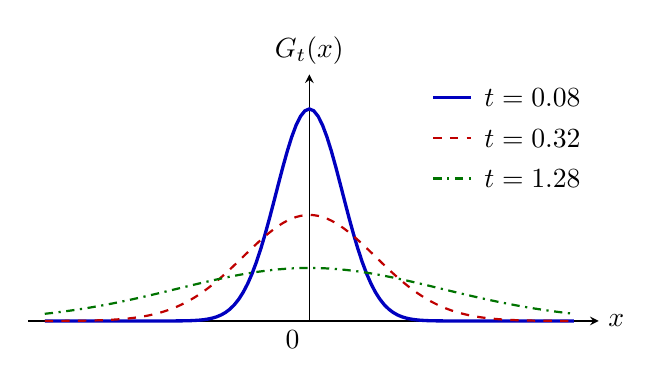
\begin{tikzpicture}[x=1.05cm,y=2.7cm,>=stealth]
	\draw[->] (-3.4,0)--(3.5,0) node[right] {\(x\)};
	\draw[->] (0,0)--(0,1.16) node[above] {\(G_t(x)\)};
	\draw[very thick,blue!75!black,domain=-3.2:3.2,samples=121]
		plot (\x,{exp(-\x*\x/.32)/sqrt(4*pi*.08)});
	\draw[thick,red!75!black,dashed,domain=-3.2:3.2,samples=121]
		plot (\x,{exp(-\x*\x/1.28)/sqrt(4*pi*.32)});
	\draw[thick,green!45!black,dash dot,domain=-3.2:3.2,samples=121]
		plot (\x,{exp(-\x*\x/5.12)/sqrt(4*pi*1.28)});
	\draw[very thick,blue!75!black] (1.5,1.05)--(1.95,1.05);
	\node[right] at (2,1.05) {\(t=0.08\)};
	\draw[thick,red!75!black,dashed] (1.5,.86)--(1.95,.86);
	\node[right] at (2,.86) {\(t=0.32\)};
	\draw[thick,green!45!black,dash dot] (1.5,.67)--(1.95,.67);
	\node[right] at (2,.67) {\(t=1.28\)};
	\node[below left] at (0,0) {\(0\)};
\end{tikzpicture}

	\caption{一维 Euclid Gaussian 核的高度与扩散尺度}
	\label{g3:fig:gaussian-scale}
\end{figure}

\Cref{g3:fig:gaussian-scale}画出三个时刻的一维模型。时间缩小为原来的四分之一时，峰值增大为两倍，集中宽度缩小为一半，而总积分仍为一。流形上将保留这种局部尺度，并用系数修正密度与曲率造成的差别。

\begin{lemma}\label{g3:lem:heat-gaussian-transport-identity}
	设 \((M^n,g)\) 为非空、\(n\ge1\) 维的光滑闭黎曼流形。在 \(d(x,y)<\rho\) 的统一法邻域中，令 \(J\) 和 \(G\) 分别由式\eqref{g3:eq:heat-normal-density}及式\eqref{g3:eq:heat-geodesic-gaussian}定义。取 \(\Delta=-\operatorname{div}\operatorname{grad}\)，定义作用于 \(x\) 变量的算子
	\[
		\mathcal T=r\partial_r+\tfrac12r\partial_r\log J.
	\]
	其中 \(r\partial_r\) 在法坐标中为 \(v^i\partial_{v^i}\)，故在对角上光滑延伸。对任意光滑的 \(a(t,x,y)\)，有
	\begin{equation}\label{g3:eq:heat-gaussian-transport-identity}
		(\partial_t+\Delta_x)(Ga)
		=G\left(\partial_ta+\Delta_xa+t^{-1}\mathcal Ta\right).
	\end{equation}
\end{lemma}
\begin{proof}
	Gauss 引理给出 \(|\mathrm d_xr|=1\)。极坐标中的体积密度为 \(r^{n-1}J_y(r\theta)\,\mathrm dr\,\mathrm d\theta\)，所以在 \(r>0\) 处
	\[
		\Delta r=-\frac{n-1}{r}-\partial_r\log J,
		\qquad \Delta(r^2)=-2n-2r\partial_r\log J.
	\]
	利用 \(\Delta(e^h)=e^h(\Delta h-|\mathrm dh|^2)\)，可得
	\[
		\frac{\partial_tG}{G}=-\frac n{2t}+\frac{r^2}{4t^2},
		\qquad
		\frac{\Delta_xG}{G}=\frac n{2t}
		+\frac{r\partial_r\log J}{2t}-\frac{r^2}{4t^2}.
	\]
	两式的 \(t^{-2}\) 项及常数 \(t^{-1}\) 项抵消。再用
	\(\Delta(Ga)=G\Delta a+a\Delta G-2\langle\mathrm dG,\mathrm da\rangle\)
	和 \(\mathrm dG/G=-r\,\mathrm dr/(2t)\)，便得结论。两边在 \(r=0\) 处均光滑，故等式也在那里成立。
\end{proof}

因而主项的修正首先是一个沿径向测地线的一阶问题。二阶算子 \(\Delta_x\) 将在后一阶才进入递推；这使系数能够逐个确定。

\subsection{运输方程与系数递推}
\label{g3:subsec:1602:02}
寻找形式为 \(G\sum_{j=0}^Nt^ju_j(x,y)\) 的近似解。代入式\eqref{g3:eq:heat-gaussian-transport-identity}，依次令 \(t^{-1},t^0,\ldots,t^{N-1}\) 的系数为零，得到\term[yunshu fangcheng]{运输方程}[transport equation]
\begin{equation}\label{g3:eq:heat-transport-recursion}
	\mathcal Tu_0=0,\qquad
	(\mathcal T+j)u_j=-\Delta_xu_{j-1}\quad(j\ge1),
	\qquad u_0(y,y)=1.
\end{equation}
最后一个条件保证对角上的质量归一化。
\symidx{\(u_j(x,y)\)：短时热核的运输系数}

\begin{proposition}\label{g3:prop:heat-transport-coefficients}
	设 \((M^n,g)\) 为非空、\(n\ge1\) 维的光滑闭黎曼流形，\(\Delta=-\operatorname{div}\operatorname{grad}\)，\(J\) 为式\eqref{g3:eq:heat-normal-density}的法坐标密度。在统一法邻域 \(d(x,y)<\rho\) 上，式\eqref{g3:eq:heat-transport-recursion}有唯一的光滑系数列。具体地，若 \(x=\exp_yv\)、\(z_s=\exp_y(sv)\)，则
	\begin{align}
		u_0(x,y)&=J_y(v)^{-1/2},\label{g3:eq:heat-u0-density}\\
		u_j(x,y)&=-J_y(v)^{-1/2}
		\int_0^1s^{j-1}J_y(sv)^{1/2}
		(\Delta_xu_{j-1})(z_s,y)\,\mathrm ds,
		\quad j\ge1.\label{g3:eq:heat-transport-integral}
	\end{align}
	特别地，
	\begin{equation}\label{g3:eq:heat-diagonal-recursion}
		u_0(y,y)=1,\qquad
		u_j(y,y)=-\frac1j(\Delta_xu_{j-1})(y,y).
	\end{equation}
\end{proposition}
\begin{proof}
	固定 \(y\) 和单位方向 \(\theta\)。把方程乘以 \(r^{j-1}J_y(r\theta)^{1/2}\)，便得到
	\[
		\partial_r\bigl(r^jJ_y(r\theta)^{1/2}u_j(\exp_y(r\theta),y)\bigr)
		=-r^{j-1}J_y(r\theta)^{1/2}
		(\Delta_xu_{j-1})(\exp_y(r\theta),y).
	\]
	当 \(j=0\) 时，右边取零，归一化给出 \(J^{1/2}u_0=1\)。当 \(j\ge1\) 时，光滑性迫使左边括号在 \(r=0\) 为零。从零积分到 \(r\)，再令积分变量为 \(rs\)，即得式\eqref{g3:eq:heat-transport-integral}。

	该积分式也证明了对角处的光滑性。若 \(u_{j-1}\) 联合光滑，其被积函数在 \((s,y,v)\in[0,1]\times\{|v|<\rho\}\) 上光滑，任意固定阶导数可移入有限区间积分，因而 \(u_j\) 联合光滑。由归纳得到全部系数。齐次方程的差解满足 \(r^jJ^{1/2}w\) 沿径向恒定；\(j\ge1\) 时光滑性使该常数为零，\(j=0\) 时由归一化也为零。这证明唯一性。最后令 \(v=0\)，利用 \(\int_0^1s^{j-1}\,\mathrm ds=1/j\)，得到对角公式。
\end{proof}

\begin{example}\label{g3:exm:flat-local-heat-coefficients}
	在一个 Euclid 开片中，\(J=1\)，所以 \(u_0=1\)、\(u_j=0\) 对所有 \(j\ge1\) 成立。同样的结论适用于平坦环面的充分小法邻域。它并不表示环面的全局热核只有一个 Gaussian 项；热流绕过全局闭路所产生的贡献，要由局部核之外的修正记录。
\end{example}

式\eqref{g3:eq:heat-transport-integral}每次只沿唯一短测地线积分，因此系数由该线附近的度量决定。在 \(v=0\) 处对该积分式求固定阶导数，右端只含 \(J\) 及上一系数的有限阶导数；逐层回代到 \(u_0=J^{-1/2}\)，可知对角上的有限阶系数只依赖有限阶度量导数。这里尚未断言无限级数收敛；接下来将对每个有限截断单独给出误差界。

\subsection{截断参数核的误差}
\label{g3:subsec:1602:03}
取 \(\chi\in C^\infty(M\times M)\)，它在 \(r<\rho/3\) 时为一，在 \(r>2\rho/3\) 时为零，且在法邻域中只依赖 \(r^2\)。定义\term[canshu he]{参数核}[parametrix]
\begin{equation}\label{g3:eq:heat-cutoff-parametrix}
	H_N(t,x,y)=\chi(x,y)G(t,x,y)\sum_{j=0}^Nt^ju_j(x,y),
	\qquad R_N=(\partial_t+\Delta_x)H_N,
\end{equation}
并在法邻域外取零。截断使它成为全局光滑核；代价是截断变化的环带上产生附加误差。

\begin{lemma}\label{g3:lem:heat-parametrix-error-bounds}
	设 \((M^n,g)\) 为非空、\(n\ge1\) 维的光滑闭黎曼流形，\(\Delta=-\operatorname{div}\operatorname{grad}\)。固定整数 \(N\ge0\)，按式\eqref{g3:eq:heat-cutoff-parametrix}取参数核 \(H_N\) 及残差 \(R_N\)。在任意固定的有限坐标覆盖及其相对紧小片上，对多重指标 \(\alpha,\beta\) 和整数 \(\ell\ge0\)，存在常数 \(C,c>0\)，使 \(0<t\le1\) 时
	\begin{align}
		|\partial_x^\alpha\partial_y^\beta\partial_t^\ell H_N|
		&\le Ct^{-n/2-(|\alpha|+|\beta|)/2-\ell}e^{-r^2/(ct)},\label{g3:eq:heat-parametrix-gaussian-bound}\\
		|\partial_x^\alpha\partial_y^\beta\partial_t^\ell R_N|
		&\le Ct^{N-n/2-(|\alpha|+|\beta|)/2-\ell}e^{-r^2/(ct)}.\label{g3:eq:heat-residual-gaussian-bound}
	\end{align}
	右端只需在核的支集附近解释；支集外左端为零。对核 \(A\) 记
	\[
		\|A\|_{\mathrm{int}}=
		\max\left\{\sup_x\int_M|A(x,y)|\,\mu_g(y),
		\sup_y\int_M|A(x,y)|\,\mu_g(x)\right\}.
	\]
	则
	\begin{equation}\label{g3:eq:heat-parametrix-integral-bounds}
		\|H_N(t)\|_{\mathrm{int}}\le C,
		\qquad \|R_N(t)\|_{\mathrm{int}}\le Ct^N.
	\end{equation}
	对每个整数 \(m\ge0\)，还成立
	\begin{equation}\label{g3:eq:heat-residual-sobolev-bound}
		\sup_y\|\partial_y^\beta R_N(t,\cdot,y)\|_{H^m(M)}
		\le Ct^{N-n/4-(m+|\beta|)/2}.
	\end{equation}
\end{lemma}
\begin{proof}
	运输方程给出确切公式
	\begin{equation}\label{g3:eq:heat-cutoff-residual}
		R_N=\chi Gt^N\Delta_xu_N
		+(\Delta_x\chi)G\sum_{j=0}^Nt^ju_j
		-2\left\langle\mathrm d_x\chi,
		\mathrm d_x\left(G\sum_{j=0}^Nt^ju_j\right)\right\rangle.
	\end{equation}
	先考察第一项。\(r^2\) 联合光滑，在对角上二阶消失，故其一次导数为 \(O(r)\)，二阶及以上的固定阶导数一致有界。对 \(e^{-r^2/(4t)}\) 求一次空间导数，增加的因子为 \(O(r/t)\)；求高阶导数得到这种因子及 \(O(t^{-1})\) 的有限乘积。把 \(r/\sqrt t\) 的任意固定幂吸收到略弱的 Gaussian 中，即
	\[
		s^a e^{-s^2/4}\le C_a e^{-s^2/8}\quad(s\ge0),
	\]
	便知每一空间导数至多损失 \(t^{-1/2}\)。一次时间导数至多损失 \(t^{-1}\)。系数及其固定阶导数在截断支集上一致有界，因此得到所需估计。

	式\eqref{g3:eq:heat-cutoff-residual}的后两项支集满足 \(r\ge\rho/3\)。在那里，对于任意 \(A,B>0\)，均有 \(t^{-A}e^{-\rho^2/(Bt)}=O(t^L)\)，其中 \(L\) 可任意指定。这由令 \(s=1/t\) 后指数压过多项式直接得到。留出一部分 Gaussian 衰减，便能吸收截断项产生的全部负幂并补足 \(t^N\)。同一计算给出 \(H_N\) 的导数估计。

	法坐标中的 \(J\) 在所用紧集上有一致上下界，故缩放 \(v=\sqrt t\,w\) 给出
	\[
		\sup_y\int_{r<\rho}e^{-r^2/(ct)}\,\mu_g(x)\le C_ct^{n/2},
	\]
	交换 \(x,y\) 后同样成立。积分点态界便得式\eqref{g3:eq:heat-parametrix-integral-bounds}。将残差的空间导数界平方后积分、开平方，得到 \(L^2\) 因子 \(t^{n/4}\)；再把 \(x\) 变量中不超过 \(m\) 阶的导数相加，便得式\eqref{g3:eq:heat-residual-sobolev-bound}。有限覆盖及光滑截断只改变常数。
\end{proof}

\begin{lemma}\label{g3:lem:heat-parametrix-initial-value}
	设 \((M^n,g)\) 为非空、\(n\ge1\) 维的光滑闭黎曼流形。对任意整数 \(N\ge0\)，式\eqref{g3:eq:heat-cutoff-parametrix}的核 \(H_N(t)\) 在 \(0<t\le1\) 时定义 \(L^2(M)\) 上一致有界的算子。若 \(f\in C^0(M)\)，则 \(t\downarrow0\) 时 \(H_N(t)f\to f\) 一致；若 \(f\in L^2(M)\)，则此收敛在 \(L^2\) 中成立。
\end{lemma}
\begin{proof}
	对任意核 \(A\)，两次使用积分估计得到
	\[
		|Af(x)|^2\le
		\left(\int|A(x,y)|\,\mu_g(y)\right)
		\left(\int|A(x,y)||f(y)|^2\,\mu_g(y)\right),
		\quad \|Af\|_2\le\|A\|_{\mathrm{int}}\|f\|_2.
	\]
	因此上一引理给出算子的一致有界性。

	对连续 \(f\)，在以 \(x\) 为中心的法坐标 \(y=\exp_xw\) 中作 \(w=\sqrt t\,z\)。被积的光滑系数在 \(w=0\) 的值为 \(u_0(x,x)J_x(0)=1\)。在任意固定的小球内，它与 \(f(y)\) 相乘后一致接近 \(f(x)\)；小球外的 Gaussian 积分一致趋零。Euclid Gaussian 总质量为一，所以零阶项趋于 \(f(x)\)，且由紧性收敛一致。其余项含 \(t^j\)、\(j\ge1\)，积分范数为 \(O(t^j)\)，因而趋零。最后用光滑函数在 \(L^2\) 中的稠密性及已证的一致算子界，得到一般初值的强收敛。
\end{proof}

\subsection{Volterra 修正及余项控制}
\label{g3:subsec:1602:04}
对于两个随时间变化的核，定义只积分过去时间的卷积
\begin{equation}\label{g3:eq:heat-volterra-convolution}
	(A*B)(t,x,y)=\int_0^t\int_M
	A(t-s,x,z)B(s,z,y)\,\mu_g(z)\,\mathrm ds.
\end{equation}
这样的积分称为 \term[Volterra juanji]{Volterra 卷积}[Volterra convolution]。\footnote{Samuel Giuseppe Vito Volterra（1860--1940），意大利数学家，研究积分方程、泛函分析及数学物理；其积分方程方法将逐次代入与连续变量中的极限联系起来。}在以下绝对收敛的范围内，Fubini 定理给出结合律。若 \(R_N\) 是 \(H_N\) 的误差，就希望找 \(\Phi_N\) 满足
\[
	\Phi_N+R_N+R_N*\Phi_N=0.
\]
逐次代入给出候选级数 \(-R_N+R_N*R_N-\cdots\)。其收敛来自时间单纯形的阶乘，而不要求 \(R_N(t)\) 在每个时刻的算子范数都小于一。

\begin{lemma}\label{g3:lem:heat-volterra-series}
	设 \((M^n,g)\) 为非空、\(n\ge1\) 维的光滑闭黎曼流形。固定整数 \(N>n/2\)，令 \(R=R_N\) 为式\eqref{g3:eq:heat-cutoff-parametrix}中非负标量 Laplace 算子的残差，按式\eqref{g3:eq:heat-volterra-convolution}定义 \(R^{*1}=R\)、\(R^{*(k+1)}=R*R^{*k}\)。对 \(0<t\le1\)，有
	\begin{align}
		\|R^{*k}(t)\|_{\mathrm{int}}
		&\le\frac{C^k(N!)^k}{(k(N+1)-1)!}
		t^{k(N+1)-1},\label{g3:eq:heat-volterra-integral-power}\\
		\|R^{*k}(t)\|_\infty
		&\le\frac{k^{n/2}C^k(N!)^k}{(k(N+1)-1)!}
		t^{k(N+1)-1-n/2}.\label{g3:eq:heat-volterra-point-power}
	\end{align}
	因此
	\begin{equation}\label{g3:eq:heat-volterra-correction}
		\Phi_N=\sum_{k=1}^\infty(-1)^kR_N^{*k}
	\end{equation}
	在 \([0,1]\times M\times M\) 上一致收敛为连续核，在 \(t=0\) 取零，并且
	\begin{equation}\label{g3:eq:heat-volterra-correction-bounds}
		\Phi_N+R_N+R_N*\Phi_N=0,
		\quad \|\Phi_N(t)\|_{\mathrm{int}}\le Ct^N,
		\quad \|\Phi_N(t)\|_\infty\le Ct^{N-n/2}.
	\end{equation}
\end{lemma}
\begin{proof}
	把 \(k\) 重卷积写成时间单纯形 \(\tau_i>0\)、\(\sum_i\tau_i=t\) 上的积分。对每个固定时间组，空间核复合的积分范数不超过各因子积分范数之积，因此不超过 \(C^k\prod_i\tau_i^N\)。反复使用
	\[
		\int_0^t(t-s)^as^b\,\mathrm ds
		=\frac{a!b!}{(a+b+1)!}t^{a+b+1}
		\quad(a,b\text{ 为非负整数})
	\]
	便得式\eqref{g3:eq:heat-volterra-integral-power}；这个一维公式可由分部积分对 \(a\) 归纳证明。

	为估计点态值，在每个时间组中选最大的 \(\tau_j\)，于是 \(\tau_j\ge t/k\)。将第 \(j\) 个核用点态界 \(C\tau_j^{N-n/2}\) 控制，其前面的核依次用行积分界，后面的核依次用列积分界，所得空间积分至多为
	\[
		C^k\tau_j^{-n/2}\prod_i\tau_i^N
		\le C^k(k/t)^{n/2}\prod_i\tau_i^N.
	\]
	再积分同一个时间单纯形即得第二个估计。这一步同时用到了行、列两种积分界。

	阶乘分母使两个级数在 \(0<t\le1\) 上绝对收敛；提取首项的 \(t^N\) 或 \(t^{N-n/2}\) 后，余下级数仍一致有界。\(R_N\) 因 \(N>n/2\) 连续延伸为零，有限重卷积也连续；上述一致收敛遂给出 \(\Phi_N\) 的连续性。利用积分界交换求和与卷积，相邻各项抵消，得到第一条恒等式。
\end{proof}

\begin{proposition}\label{g3:prop:heat-local-corrected-kernel}
	设 \((M^n,g)\) 为非空、\(n\ge1\) 维的光滑闭黎曼流形，\(\Delta=-\operatorname{div}\operatorname{grad}\)。对任意整数 \(N>n/2\)，取式\eqref{g3:eq:heat-cutoff-parametrix}的参数核 \(H_N\) 及式\eqref{g3:eq:heat-volterra-correction}的核 \(\Phi_N\)，令
	\begin{equation}\label{g3:eq:heat-local-corrected-kernel}
		\widetilde K_N=H_N+H_N*\Phi_N.
	\end{equation}
	它在 \((0,1]\times M\times M\) 上连续，满足分布方程
	\((\partial_t+\Delta_x)\widetilde K_N=0\)，并且
	\begin{equation}\label{g3:eq:heat-volterra-remainder}
		\|\widetilde K_N(t)-H_N(t)\|_\infty
		\le Ct^{N+1-n/2},\qquad
		\|\widetilde K_N(t)-H_N(t)\|_{\mathrm{int}}
		\le Ct^{N+1}.
	\end{equation}
	对任意 \(f\in L^2(M)\)，\(\widetilde K_N(t)f\) 连续延伸到 \(t=0\)，其 \(L^2\) 初值为 \(f\)。
\end{proposition}
\begin{proof}
	积分范数估计直接来自
	\(\int_0^t\|H_N(t-s)\|_{\mathrm{int}}
	\|\Phi_N(s)\|_{\mathrm{int}}\,\mathrm ds\le Ct^{N+1}\)。
	点态估计把积分分成 \(s\le t/2\) 和 \(s\ge t/2\)。在第一段，用 \(H_N(t-s)\) 的上确界和 \(\Phi_N(s)\) 的列积分界；在第二段，用 \(H_N(t-s)\) 的行积分界和 \(\Phi_N(s)\) 的上确界。于是
	\[
		|H_N*\Phi_N|
		\le C\int_0^{t/2}(t-s)^{-n/2}s^N\,\mathrm ds
		+C\int_{t/2}^ts^{N-n/2}\,\mathrm ds
		\le Ct^{N+1-n/2}.
	\]
	在固定的正时间附近，避开两个积分端点后被积核连续且有界；接近 \(s=0\) 的部分由上述界控制，接近 \(s=t\) 的长度为 \(\varepsilon\) 的部分由 \(H_N\) 的行积分界控制为 \(C\varepsilon\)。先截去端点，再让 \(\varepsilon\downarrow0\)，证明卷积连续。相同论证与积分范数界也给出作用于 \(L^2\) 后的正时间连续性，初值则由\cref{g3:lem:heat-parametrix-initial-value}得到。

	为了验证方程，将 \(H_N,R_N\) 在负时间延为零。对任意光滑紧支集的双变量时空测试函数 \(\psi(t,x,y)\)，沿法坐标作与初值引理相同的缩放，可得
	\[
		\int_{M\times M}H_N(\varepsilon,x,y)\psi(\varepsilon,x,y)
		\,\mu_g(x)\mu_g(y)
		\longrightarrow\int_M\psi(0,x,x)\,\mu_g(x).
	\]
	具体说，在对角附近令 \(y=\exp_x(\sqrt\varepsilon\,v)\)，光滑系数一致趋于 \(\psi(0,x,x)\)，外部尾项由 Gaussian 控制；高阶项含正幂 \(\varepsilon^j\)，因而消失。于是以 \(\psi\) 配对，在 \(t\ge\varepsilon\) 上对时间分部积分，再令 \(\varepsilon\downarrow0\)，得到
	\[
		(\partial_t+\Delta_x)H_N
		=\delta_0(t)I+R_N
	\]
	的核分布恒等式。这里 \(I\) 的核是对角上的单位分布；残差在零附近可积，所以取极限合法。再与 \(\Phi_N\) 卷积，Fubini 定理和前述绝对积分界给出
	\[
		(\partial_t+\Delta_x)(H_N*\Phi_N)
		=\Phi_N+R_N*\Phi_N.
	\]
	这也可先让测试函数避开时间端点，再按同样估计取极限。因此 \(t>0\) 时，\(\widetilde K_N\) 的残差为 \(R_N+\Phi_N+R_N*\Phi_N=0\)。整个计算在分布意义下进行，未对零时间处奇异的 Gaussian 核直接求导后交换积分。
\end{proof}

\subsection{局部构造与谱核的一致性}
\label{g3:subsec:1602:05}
现在已有一个满足正确方程和初值的连续核。对 \(f\in L^2(M)\)，\cref{g3:thm:heat-spectral-solution}的唯一性立即给出
\[
	\widetilde K_N(t)f=T_tf\qquad(0<t\le1).
\]
两侧的连续积分核必相同：固定 \(x\) 后，核之差与所有 \(L^2\) 函数积分为零，取该行之差的复共轭作测试即可。因此 \(\widetilde K_N=K\)，其中 \(K\) 是上一节的谱核。这同时证明了它不依赖所选截断函数或足够大的 \(N\)，并且在正时间联合光滑。

\ProseParagraphBreak

下一定理给出全部有限阶导数的误差。其证明先取比目标阶数更高的截断，得到一个很小的光滑误差，然后把多取的有限项减回去。这样可以分别控制零时间的可积性和最终余项的精确阶数。

\begin{theorem}\label{g3:thm:heat-parametrix-expansion}
	设 \((M^n,g)\) 为非空、\(n\ge1\) 维的光滑闭黎曼流形，\(K\) 是非负算子 \(\Delta=-\operatorname{div}\operatorname{grad}\) 的热核。取上述法邻域、截断函数及运输系数。对每个整数 \(N\ge0\)，有
	\begin{equation}\label{g3:eq:heat-parametrix-expansion}
		K(t,x,y)=\chi(x,y)(4\pi t)^{-n/2}e^{-r^2/(4t)}
		\sum_{j=0}^Nt^ju_j(x,y)+E_N(t,x,y).
	\end{equation}
	对任意固定的多重指标 \(\alpha,\beta\) 和整数 \(\ell\ge0\)，在有限坐标覆盖的相对紧小片上存在一致常数，使
	\begin{equation}\label{g3:eq:heat-parametrix-derivative-remainder}
		|\partial_x^\alpha\partial_y^\beta\partial_t^\ell E_N(t,x,y)|
		\le Ct^{N+1-n/2-(|\alpha|+|\beta|)/2-\ell},
		\qquad 0<t\le1.
	\end{equation}
	特别地，以下对角余项对 \(x\in M\) 一致：
	\begin{equation}\label{g3:eq:heat-diagonal-uniform-remainder}
		K(t,x,x)=(4\pi t)^{-n/2}\sum_{j=0}^Nt^ju_j(x,x)
		+O(t^{N+1-n/2}).
	\end{equation}
\end{theorem}
\begin{proof}
	先说明高阶残差如何控制误差。由\cref{g3:thm:elliptic-spectral-sobolev}，对每个偶数 \(m=2q\)，算子 \(T_t\) 在 \(H^m\) 上一致有界，\(0\le t\le1\)：在等价的谱范数中，它只把各系数乘以 \(e^{-t\lambda_j}\le1\)。

	若整数 \(L\) 足够大，使式\eqref{g3:eq:heat-residual-sobolev-bound}的右端在零附近可积，则令
	\begin{equation}\label{g3:eq:heat-high-remainder-duhamel}
		W_L(t,\cdot,y)=-\int_0^tT_{t-s}R_L(s,\cdot,y)\,\mathrm ds.
	\end{equation}
	这是 \(H^m\) 中的积分，且初值为零。为核对方程，将被积函数投到特征函数 \(\phi_j\) 上，所得系数为
	\[
		-\int_0^te^{-(t-s)\lambda_j}
		(R_L(s,\cdot,y),\phi_j)\,\mathrm ds.
	\]
	该系数满足导数加 \(\lambda_j\) 倍自身等于残差系数的负值。有限谱和满足非齐次方程，利用 \(L^1((0,1);H^m)\) 的残差控制，取极限即得 \((\partial_t+\Delta)W_L=-R_L\) 的分布等式。

	取 \(L>n/2\)。已经证明的式\eqref{g3:eq:heat-volterra-remainder}说明 \(E_L=K-H_L\) 对每个固定 \(y\) 在 \(t=0\) 有零 \(L^2\) 初值；它满足同一非齐次方程。因此 \(E_L-W_L\) 是零初值的 \(L^2\) 连续齐次分布解，唯一性给出 \(E_L=W_L\)。对 \(y\) 求固定阶导数也可以移入式\eqref{g3:eq:heat-high-remainder-duhamel}，因为相应的 \(H^m\) 范数有统一可积上界。于是
	\begin{equation}\label{g3:eq:heat-high-remainder-sobolev}
		\sup_y\|\partial_y^\beta E_L(t,\cdot,y)\|_{H^m}
		\le Ct^{L+1-n/4-(m+|\beta|)/2}.
	\end{equation}

	现在固定 \(N,\alpha,\beta,\ell\)。选择偶数 \(m>|\alpha|+2\ell+n/2\)，再选择整数
	\[
		L\ge N+m+|\beta|+2\ell+n+2.
	\]
	这些选择保证以上积分可积，也保证式\eqref{g3:eq:heat-high-remainder-sobolev}的指数不小于目标指数
	\(N+1-n/2-(|\alpha|+|\beta|)/2-\ell\)。由高阶 Sobolev 嵌入，它控制 \(E_L\) 的 \(x\) 变量中不超过 \(|\alpha|+2\ell\) 阶的导数。时间导数用已经成立的方程递推：
	\[
		\partial_t^\ell E_L=(-\Delta)^\ell E_L
		-\sum_{j=0}^{\ell-1}(-\Delta)^{\ell-1-j}\partial_t^jR_L
		\qquad(\ell\ge1).
	\]
	第一项由刚才的 Sobolev 界控制。对求和项使用式\eqref{g3:eq:heat-residual-gaussian-bound}，其空间阶数为 \(|\alpha|+2(\ell-1-j)\)，时间阶数为 \(j\)，故指数至少为
	\(L+1-n/2-(|\alpha|+|\beta|)/2-\ell\)，也足够。这里全在正时间的光滑函数上运算。

	最后写
	\[
		E_N=E_L+(H_L-H_N)
		=E_L+\chi G\sum_{j=N+1}^Lt^ju_j.
	\]
	有限和的每项经同样的 Gaussian 导数估计，恰好满足式\eqref{g3:eq:heat-parametrix-derivative-remainder}。合并两部分即得结论。对角上 \(\chi=1\)、\(r=0\)，令 \(\alpha=\beta=\ell=0\) 得最后一式。
\end{proof}

这一展开是逐个 \(N\) 的渐近断言，不需要 \(\sum_{j\ge0}t^ju_j\) 收敛。离开对角的任意固定邻域，显式 Gaussian 项连同所有固定阶导数均小于任意幂；再任意提高 \(N\)，可知真正热核在该区域也具有同样的任意幂衰减。对角系数则保存了短时仍然可见的几何信息。

\ProseParagraphBreak

后续的 Hodge 与 Dirac 问题需要丛值版本。下面把新增的几何步骤写出；时间卷积与余项估计仍是已经证明的有限维范数估计。

\begin{proposition}\label{g3:prop:laplace-type-heat-parametrix}
	设 \((M^n,g)\) 为非空、\(n\ge1\) 维的光滑闭黎曼流形，\(E\to M\) 为正秩光滑 Hermitian 丛，\(\nabla\) 为相容联络，\(V\) 为光滑自伴丛自同态。假设 \(P=\nabla^*\nabla+V\) 非负。令 \(\tau(x,y):E_y\to E_x\) 为沿唯一短径向测地线的平行移动，则 \(P\) 的热核有式\eqref{g3:eq:heat-parametrix-expansion}及式\eqref{g3:eq:heat-parametrix-derivative-remainder}的丛值版本，其中乘积解释为纤维映射复合，导数在有限光滑平凡化中计算。其系数满足
	\begin{align}
		u_0^E(x,y)&=J(x,y)^{-1/2}\tau(x,y),\label{g3:eq:bundle-heat-leading-coefficient}\\
		\left(r\nabla_{\partial_r}+\tfrac r2\partial_r\log J+j\right)u_j^E
		&=-P_xu_{j-1}^E\qquad(j\ge1),\label{g3:eq:bundle-heat-transport}\\
		u_1^E(y,y)&=u_1(y,y)I_{E_y}-V(y).\label{g3:eq:bundle-heat-first-potential}
	\end{align}
	这里 \(u_1\) 是同一度量的标量系数。
\end{proposition}
\begin{proof}
	对标量 \(G\) 与丛值 \(a\)，相容联络的乘法公式为
	\[
		P(Ga)=GPa+(\Delta G)a-2\nabla_{\operatorname{grad}G}a.
	\]
	所以 Gaussian 计算只需把径向普通导数换为协变导数。由于 \(\nabla_{\partial_r}\tau=0\)，零阶运输方程给出所述 \(u_0^E\)。令 \(x=\exp_yv\)、\(z_s=\exp_y(sv)\)，高阶解具体为
	\[
		u_j^E(x,y)=-J(x,y)^{-1/2}\tau(x,y)
		\int_0^1s^{j-1}J(z_s,y)^{1/2}\tau(z_s,y)^{-1}
		(P_xu_{j-1}^E)(z_s,y)\,\mathrm ds.
	\]
	平行移动对端点光滑依赖，所以此式给出联合光滑的系数；径向常微分方程和对角正则性再次给出唯一性。固定有限平凡化，矩阵的算子范数满足 \(\|AB\|\le\|A\|\|B\|\)，且纤维秩有限。因此残差估计、行列积分界、时间单纯形估计与收敛级数逐项成立。上一节的丛值谱核具有同一 \(L^2\) 连续分布解唯一性；第十三章的丛值谱范数又给出 \(H^{2q}\) 上的一致有界性。因此识别及高阶余项证明的每一步均适用。

	最后核算 \(u_1^E\)。固定 \(y\)，从 \(E_y\) 的正交标架作径向平行移动。在所得标架中，\(\tau\) 的矩阵为常值 \(I\)，联络矩阵 \(A_i(v)\) 满足 \(v^iA_i(v)=0\)。一次微分后在 \(v=0\) 取值，得 \(A_i(0)=0\)；二次微分给出 \(\partial_iA_j(0)+\partial_jA_i(0)=0\)，特别有 \(\sum_i\partial_iA_i(0)=0\)。法坐标在中心的 Christoffel 符号也为零，故 \((\nabla^*\nabla\tau)(y,y)=0\)。又因 \(\mathrm d_xJ(y,y)=0\)，乘法公式给出
	\[
		(P_xu_0^E)(y,y)=(\Delta_xJ^{-1/2})(y,y)I+V(y).
	\]
	在一阶运输方程的对角上取值，再与标量公式\eqref{g3:eq:heat-diagonal-recursion}比较，即得式\eqref{g3:eq:bundle-heat-first-potential}。
\end{proof}

下一节的\cref{g3:prop:heat-diagonal-first-coefficients}将由法坐标体积密度算出 \(u_1(x,x)=\operatorname{Scal}(x)/6\)。因此丛值一阶系数为 \(\operatorname{Scal}(x)I/6-V(x)\)：度量的体积扩张与算子的零阶势分别贡献这两个项。
% 纲要条目排为编号小节标题，并进入目录与书签；说明段仍保留于纲要注释中。
